\chapter{Custom Plots}
\label{sec:customplots}
The custom plots form a powerful mechanism allowing the user to freely create and configure additional plots. The focus of this chapter lies on how to create and customize said custom plots.

\section{Location}
All custom plot code should be written to the respective custom-config files located in the dna/config directory. These files hold all default custom plots aswell as extensive examples.

\section{Syntax}
For each type of custom plot there is a default prefix. See table \ref{tab:prefixes}. For each prefix, there is a field called 
which defines the respective plots. For example:
defines, that there are two custom runtime plots, called R1 and R2. These identifiers will be used further to specify the plots. See the examples in section \ref{sec:example} for further details.

\begin{table}[h]
\centering
\begin{tabular}[h]{|l|l|}\hline
	\textbf{Prefix} & \textbf{Type}\\
	\hline
	CUSTOM\_ & General custom plot which can contain any sort of values.\\
	\hline
	RT\_ & Runtime plot.\\
	\hline
	ST\_ & Statistics plot.\\
	\hline
	MV\_ & Metric-Value plot.\\
	\hline
	MD\_ & Metric-Distribution plot.\\
	\hline
	MNVL\_ & Metric-nodeValueList plot.\\
	\hline
\end{tabular}
\caption{Prefixes for custom plots.}
\label{tab:prefixes}
\end{table}

\subsection{Example}
\label{sec:example}
The code snippet below shows an example on how one could specify a custom plot, which will plot the inDegreeDistribution of a metric called DegreeDistributionR as a cumulative distribution function (cdf). 

\begin{figure}
\begin{lstlisting}
MD_PLOTS = D1
MD_1_FILENAME = distributionPlot1
MD_D1_VALUES = DegreeDistributionR~inDegreeDistribution
MD_D1_TYPE = distANDcdf
MD_D1_KEY = off
\end{lstlisting}
\caption{Example of a custom distribution plot.}
\label{ex:1}
\end{figure}

Note the syntax used in the definition. The prefix MD{\_} derives from the prefix for metric distribution plots and is followed by the identifier D1, which itself is always followed by a suffix. The suffix {\_}VALUES is the only mandatory field and defines which values will be included in the plot. A list of all available suffixes can be found in table \ref{tab:suffixes}. The {\_}KEY field is used to configure the legend in gnuplot. Here it is turned off for a clear result.

\begin{figure} [h]
\centering
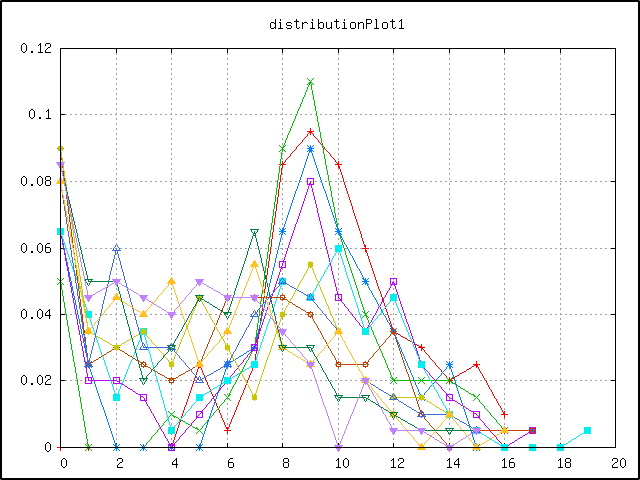
\includegraphics [scale=0.65] {images/dist}
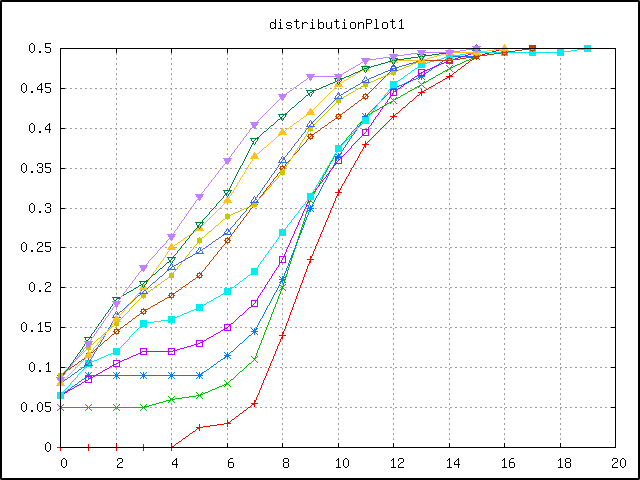
\includegraphics [scale=0.65] {images/distCDF}
\caption{Resulting plots from example \ref{ex:1}.}
\label{fig:33}
\end{figure}


\begin{table}[hp]
\centering
\begin{tabular}[h]{|l|l|}\hline
	\textbf{Suffix} & \textbf{Type}\\
	\hline
	{\_}FILENAME & Filename of the resulting script and plot.\\
	\hline
	{\_}VALUES & Defines the values contained in the plot.\\
	\hline
	{\_}DOMAIN & Defines a domain for the plot. If set all values that are being\\
	& defined without domain will be treated as if they had this domain.\\
	\hline
	{\_}TITLE & Title of the plot.\\
	\hline
	{\_}CDF & If the plot should be plotted as cdf.\\
	& Possible values: true, false, both.\\
	\hline
	{\_}DATETIME & If set datetime will be used for timestamps on the x-axis.\\
	& Uses gnuplot datetime.\\
	\hline	
	{\_}LOGSCALE & Sets if x and/or y axis should have logarithmic scaling.\\
	& Possible values: x, y, xy\\
	\hline
	{\_}XLABEL & Sets the label of the x-axis.\\
	\hline
	{\_}YLABEL & Sets the label of the y-axis.\\
	\hline
	{\_}XOFFSET & Sets an offset for the x-axis.\\
	\hline
	{\_}YOFFSET & Sets an offset for the y-axis.\\
	\hline
	{\_}XRANGE & Sets the range of the x-axis.\\
	\hline
	{\_}YRANGE & Sets the range of the y-axis.\\
	\hline
	{\_}XTICS & Sets the tics which will be shown on the x-axis. See gnuplot\\
	& documentation for futher details.\\
	\hline
	{\_}YTICS & Sets the tics which will be shown on the y-axis. See gnuplot\\
	& documentation for futher details.\\
	\hline
	{\_}TYPE & Only available for distribution plots. Sets how the distribution \\
	& will be plotted.\\
	\hline
	{\_}STYLE & Style of the plot. Possible values: lines, dots, points, linespoint,\\
	&	impulses, steps, boxes, candlesticks, yerrorbars, fillsteps, filledcurves\\
	\hline
	{\_}ORDER & Only available for nodevaluelist plots. Sets how the\\
	&	nodevaluelists should be ordered. Possible values:\\
	&	ascending, descending.\\
	\hline
	{\_}ORDERBY & Only available for nodevaluelist plots. Sets by\\
	&	which value the nodevaluelists should be ordered. \\
	&	Possible values: index, average, median, minimum, maximum,\\
	&	variance, varianceLow, varianceUp, confidenceLow, confidenceUp.\\
	\hline
	{\_}SORTMODE & Sets which mode will be used for sorting. Possible values are:\\
	& NONE, LIST\_ FIRST, LIST\_ LAST, ALPHABETICAL,\\
	& ALPHABETICAL\_ LIST\_ FIRST, ALPHABETICAL\_ LIST\_ LAST.\\
	\hline
	{\_}SORTLIST & Sets a list of values that will be handled special in the\\ 
	& sorting process.\\
	\hline
\end{tabular}
\caption{List of all suffixes.}
\label{tab:suffixes}
\end{table}

\subsection{Domains}
In order to adress a value in a unique way, it is neccessary to know where it is stored. For example two different metrics “metric1“ and “m2“ may calculate the number of edges in a graph and store it as a value called “edges“. For this case the domain got introduced. It can either be the name of a metric or a static string. The following shows how the two different values can be adressed:

\centerline{metric1\textasciitilde edges}
\centerline{m2\textasciitilde edges}

Note the delimiter \textasciitilde .
As seen in the former example \ref{sec:example}, the “inDegreeDistribution “ has been adressed with

\centerline{DegreeDistributionR\textasciitilde inDegreeDistribution	,}

where “DegreeDistributionR“ is the domain. Runtimes and statistics can be adressed with static domains. For a list of all staticly defined domains, check table \ref{tab:domains}. Note that for custom plots with the prefix ST{\_} and RT{\_} it is not necessary to set domains, as these are statistics or runtime plots by definition and values from other domains are not allowed.

\begin{table} [h]
\centering
\begin{tabular}[h]{|l|l|}\hline
	\textbf{Prefix} & \textbf{Type}\\
	\hline
	statistics & Domain of statistical values.\\
	\hline
	runtimes & Domain of runtimes. Can be used to adress either.\\
	& metric runtimes or general runtimes.\\
	\hline
	metric{\_}runtimes & Domain of metric runtimes.\\
	\hline
	general{\_}runtimes & Domain of general runtimes.\\
	\hline
\end{tabular}
\caption{List of static domains.}
\label{tab:domains}
\end{table}

\section{Wildcards}
The described way to define custom plots is very restricted in regards of dynamic use. In each plot the value‘s have to be explicitly defined. There are several cases where this might not be convenient. For example the user wants a plot, which shows the runtimes of all current metrics for arbitrary series‘. Wildcards * provide a sophisticated way to deal with such cases. The code in figure \ref{fig:36} creates a plot with the runtimes of all used metrics, in this case DiceDirectedR-out, DicreDirectedU-out and DegreeDistributionR, and additionally the total runtime. Note that wildcards can not be used to replace domains. Additionally only one wildcard might be used in the same value definition.

\begin{figure} [h]
\centering
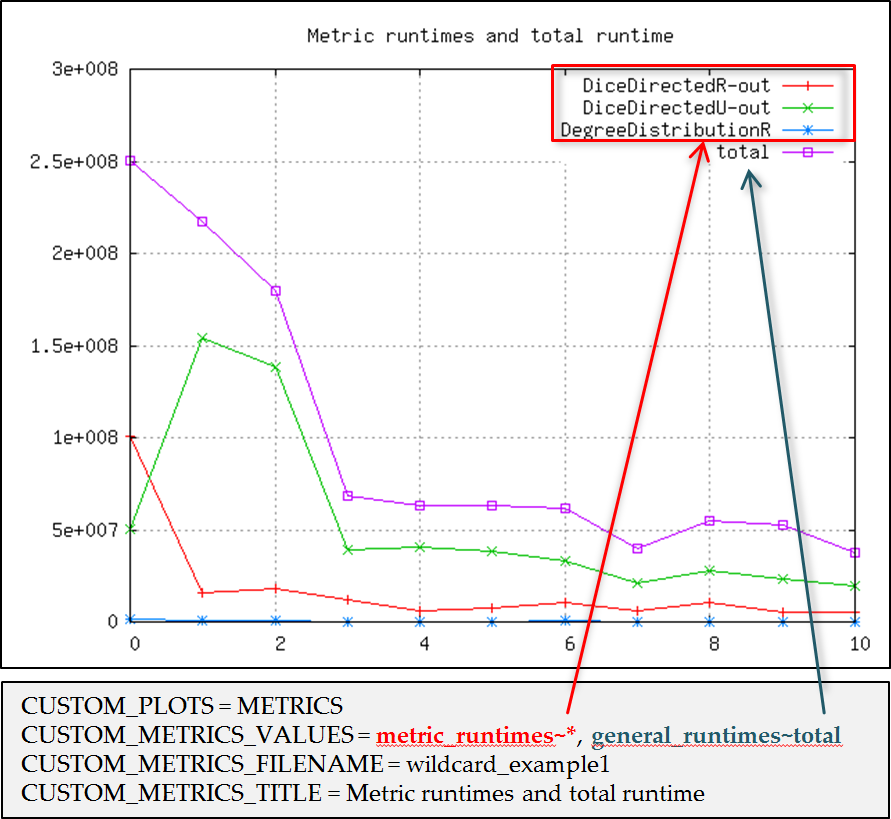
\includegraphics [scale=0.5] {images/36}
\caption{Example plot with wildcards.}
\label{fig:36}
\end{figure}

\section{Mathematical expressions}
The modification of plotted data can often be necessary. For example the runtimes are measured in nanoseconds. Mathematical expressions can be used to transform these into seconds. Example \ref{fig:37} shows how one could do that. Note the double point : , which signals the DNA that it is dealing with a mathematical expression. Variables are <domain>~<value> pairs surrounded by \$ . Note that it is possible to add multiple variables to one expression. This allows to also combine different values. In addition wildcards can be used in mathematical expressions. For each value the wildcard will be replaced by the respective value and then calculated.

\begin{figure} [h]
\centering
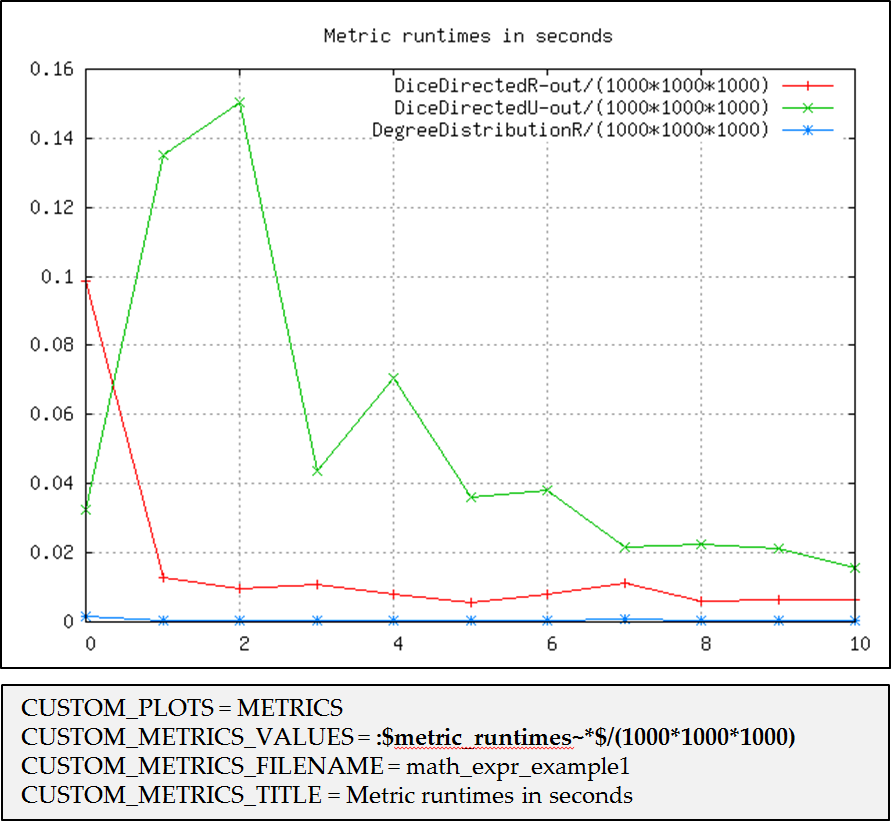
\includegraphics [scale=0.5] {images/37}
\caption{Using mathematical expressions and wildcards to plot metric runtimes in seconds.}
\label{fig:37}
\end{figure}

The plot in figure \ref{fig:37} achieved exactly what we wanted. The runtimes are being devided by 10*9 and therefore appear as seconds. However, there is no label on the y-axis indicating that we are dealing with seconds. By adding a line defining the {\_}YLABEL, we can set it to “sec“, see figure \ref{fig:38}.

\begin{figure} [h]
\centering
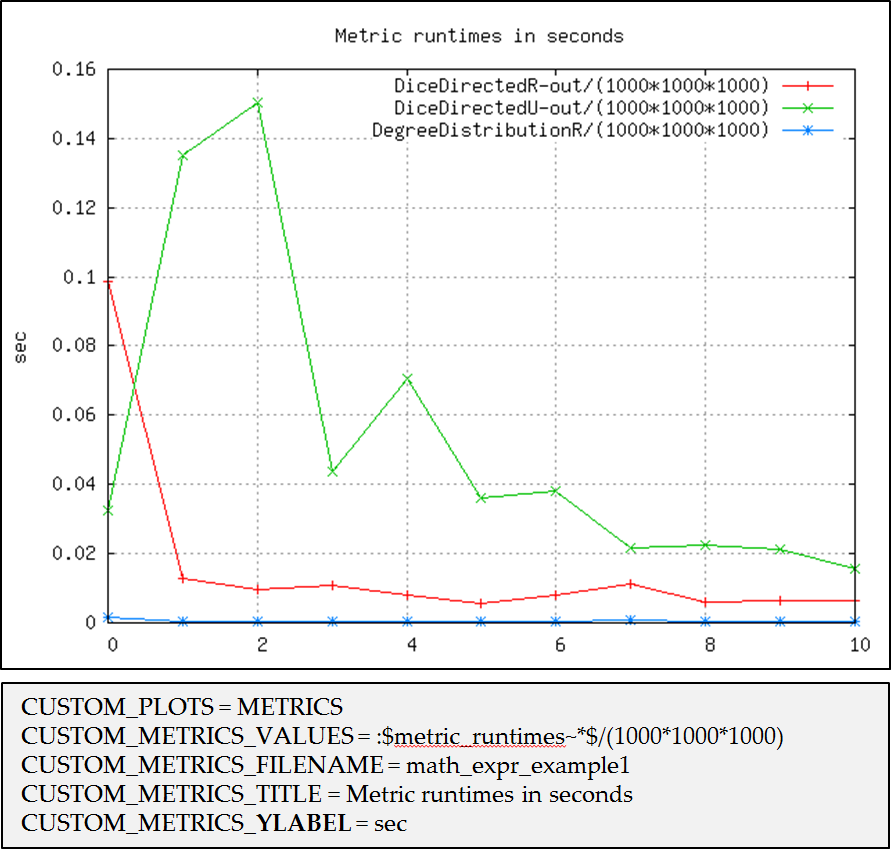
\includegraphics [scale=0.5] {images/38}
\caption{Adding a label to the y-axis.}
\label{fig:38}
\end{figure}

Now the y-axis is labeled and the plot got more reasonable. But still, the lines hold the entire mathematical equations in their labels. In order to clean up the plot we can give the mathematical expression a name by adding a string before the double point. The example code in figure \ref{fig:39} assigns “ab c“ as the expressions name.

\begin{figure} [h]
\centering
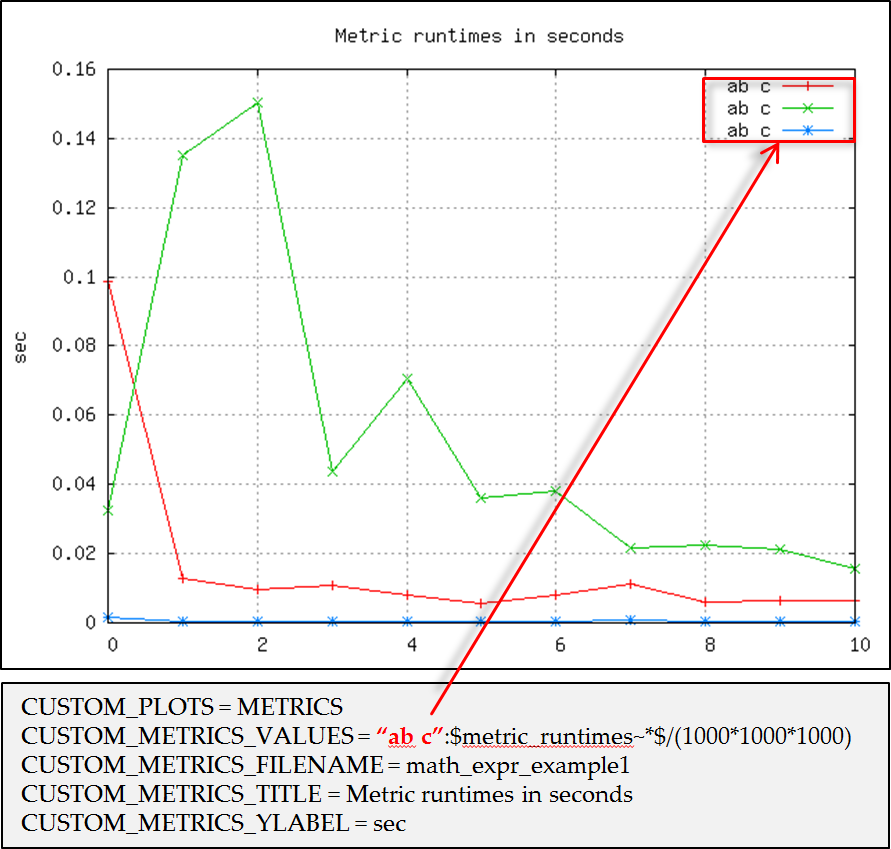
\includegraphics [scale=0.5] {images/39}
\caption{Assigning a name to the math. expression.}
\label{fig:39}
\end{figure}

As we can see, all lines created by the expression have been named “ab c“. However, especially when dealing with wildcards, this behaviour might not be desirable, because for multiple values it is not clear which line represents which value. More sophisticated naming schemes can be created by inserting a wildcard surrounded by \$ into the name string. The wildcard will be replaced by the name of the respective value. See figure \ref{fig:310} on the next page for an example.

\begin{figure} [h]
\centering
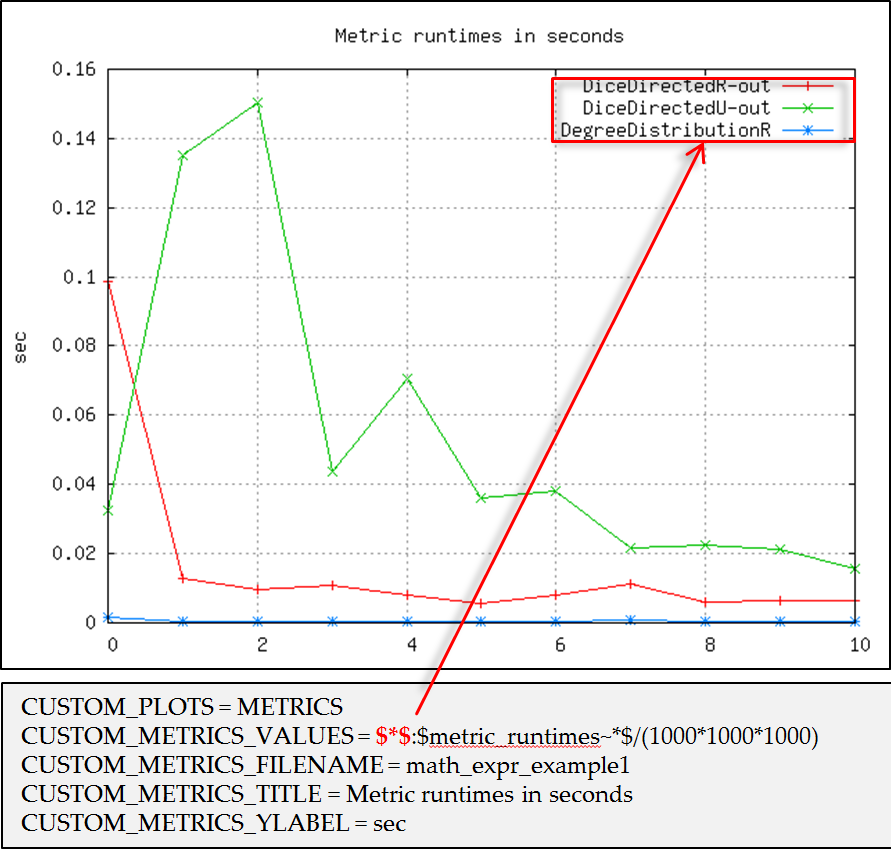
\includegraphics [scale=0.5] {images/310}
\caption{Using wildcards in expression names.}
\label{fig:310}
\end{figure}

\section{Functions}
The above described mathematical expressions only allow to transform given values. In order to investigate scaling or complexity problems it can be useful to add chosen functions to the plot. This is possible with straight-forward function definitions in the values field. The example in figure \ref{fig:311} extends the in the last section introduced mathematical expression example by adding a function. A more sophisticated example of function definitions can be found on the following page.

\begin{figure} [h]
\centering
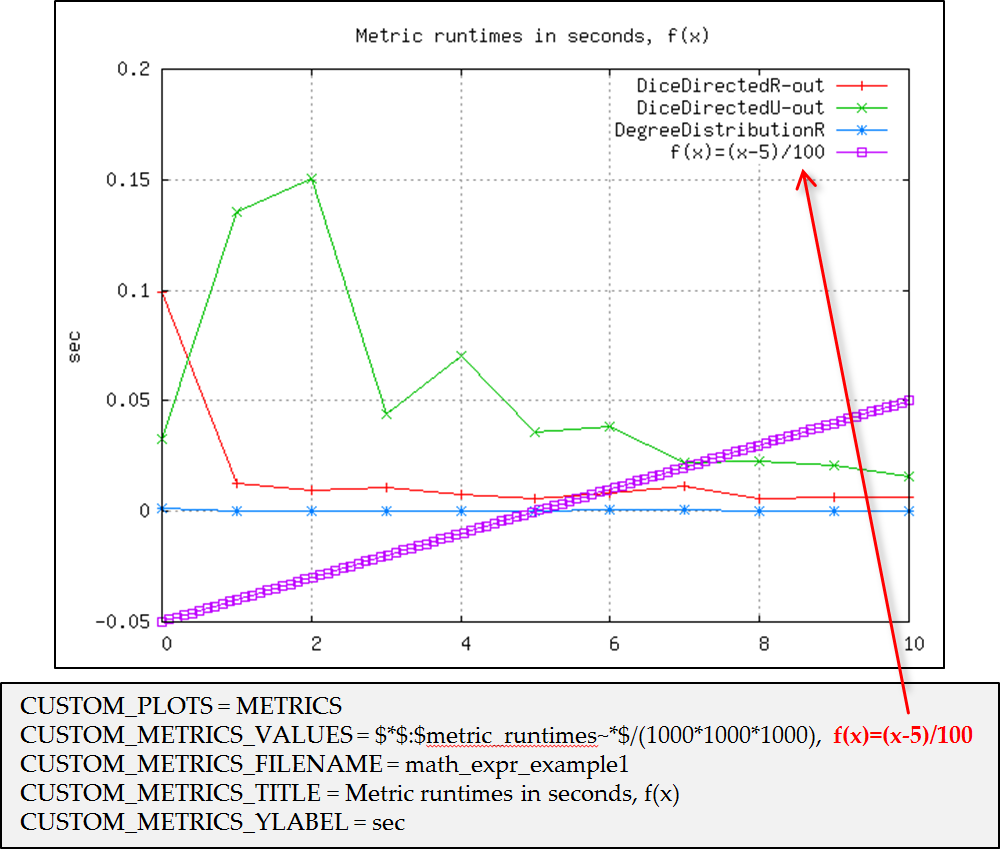
\includegraphics [scale=0.5] {images/311}
\caption{Adding a mathematical function to the plot.}
\label{fig:311}
\end{figure}

\begin{figure} [h]
\centering
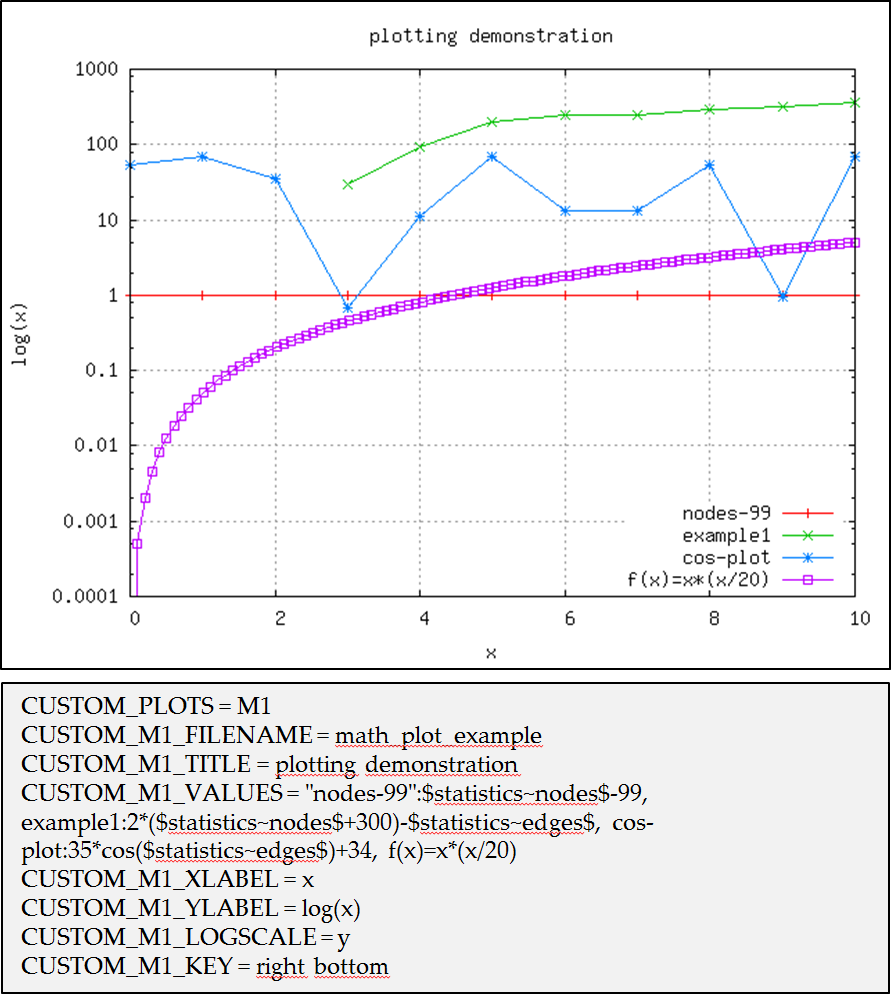
\includegraphics [scale=0.5] {images/312}
\caption{Extended example demonstrating possible function definitions.}
\label{fig:312}
\end{figure}